%%% LaTeX Template: Article/Thesis/etc. with colored headings and special fonts
%%%
%%% Source: http://www.howtotex.com/
%%% Feel free to distribute this template, but please keep to referal to http://www.howtotex.com/ here.
%%% February 2011

%%%%% Preamble
\documentclass[10pt,a4paper]{article}

\usepackage[T1]{fontenc}
\usepackage[bitstream-charter]{mathdesign}

\usepackage[utf8]{inputenc}							% Input encoding
\usepackage{amsmath}									% Math

\usepackage{xcolor}
\definecolor{bl}{rgb}{0.0,0.2,0.6} 

\definecolor{background-image}{rgb}{1.0,0.9,0.7} 

% Translating the section, part, ... names into French
\usepackage[french]{babel}

% Setup the margins
\usepackage{geometry}
\newgeometry{margin=2cm}

% Customize the hyperlinks
\usepackage{hyperref}
\hypersetup{
    bookmarks=true,         % show bookmarks bar?
    unicode=false,          % non-Latin characters in Acrobat’s bookmarks
    pdftoolbar=true,        % show Acrobat’s toolbar?
    pdfmenubar=true,        % show Acrobat’s menu?
    pdffitwindow=false,     % window fit to page when opened
    pdfstartview={FitH},    % fits the width of the page to the window
    pdftitle={My title},    % title
    pdfauthor={Author},     % author
    pdfsubject={Subject},   % subject of the document
    pdfcreator={Creator},   % creator of the document
    pdfproducer={Producer}, % producer of the document
    pdfkeywords={keyword1} {key2} {key3}, % list of keywords
    pdfnewwindow=true,      % links in new window
    colorlinks=true,       % false: boxed links; true: colored links
    linkcolor=bl,          % color of internal links (change box color with linkbordercolor)
    citecolor=green,        % color of links to bibliography
    filecolor=magenta,      % color of file links
    urlcolor=bl           % color of external links
}

% For getting the caption on the side of an image
\usepackage{calc}
\usepackage{graphicx}
\usepackage{floatrow}
\floatsetup{style=ruled,footposition=caption}

\newcommand{\myfig}[2]{
\begin{figure}[htbp]
\floatbox[{\capbeside\thisfloatsetup{capbesideposition={right,top},capbesidewidth=4cm}}]{figure}[\FBwidth]
         {\caption{#2}\label{fig:#1}}
         {\includegraphics[width=5cm]{#1}}
\end{figure}
}


%\usepackage{sidecap}

\usepackage{sectsty}
\usepackage[compact]{titlesec} 
\allsectionsfont{\color{bl}\scshape\selectfont}

%%%%% Definitions
% Define a new command that prints the title only
\makeatletter							% Begin definition
\def\printtitle{%						% Define command: \printtitle
    {\color{bl} \centering \huge \sc \textbf{\@title}\par}}		% Typesetting
\makeatother							% End definition

\title{Machine Learning \\ 
		\large \vspace*{-10pt} Notes on A. Ng lectures\vspace*{10pt}}

% Define a new command that prints the author(s) only
\makeatletter							% Begin definition
\def\printauthor{%					% Define command: \printauthor
    {\centering \small \@author}}				% Typesetting
\makeatother							% End definition

\author{%
	Jérémy Fix \\
	Jeremy.Fix@Supelec.fr \\
	\vspace{20pt}
	}

% Custom headers and footers
\usepackage{fancyhdr}
	\pagestyle{fancy}					% Enabling the custom headers/footers
\usepackage{lastpage}	
	% Header (empty)
	\lhead{}
	\chead{}
	\rhead{}
	% Footer (you may change this to your own needs)
	\lfoot{\footnotesize }
	\cfoot{}
	\rfoot{\footnotesize page \thepage\ / \pageref{LastPage}}	% "Page 1 of 2"
	\renewcommand{\headrulewidth}{0.0pt}
	\renewcommand{\footrulewidth}{0.4pt}

% Change the abstract environment
\usepackage[runin]{abstract}			% runin option for a run-in title
\setlength\absleftindent{30pt}		% left margin
\setlength\absrightindent{30pt}		% right margin
\abslabeldelim{\quad}						% 
\setlength{\abstitleskip}{-10pt}
\renewcommand{\abstractname}{}
\renewcommand{\abstracttextfont}{\color{bl} \small \slshape}	% slanted text


% Pour gérer les lettrines
\usepackage{lettrine}

%%%%%%%%%%%%%%%%%%%%%%%%%%%%%%%%%%%%%%%%%%%%%%%%%%%%%%%%%%%%%%%%%%%%%%%%%%
%%% Start of the document
%%%%%%%%%%%%%%%%%%%%%%%%%%%%%%%%%%%%%%%%%%%%%%%%%%%%%%%%%%%%%%%%%%%%%%%%%%
\begin{document}
%%% Top of the page: Author, Title and Abstact
\printtitle 

\printauthor

\begin{abstract}
Notes on the Machine Learning lectures of A. Ng.
\end{abstract}

\tableofcontents

\pagebreak

\section{Linear regression with one or multiple variables}

\section{Logistic Regression}

We focus on classification problems for which the output $y$ is binary
(bi-class classification problem, later on, we will speak about
multiclass classification): $y \in \{0, 1\}$. We call class-0
the negative class and class-1 the positive class but these are just
arbitrary names. For example, one may seek to learn to classify a
tumor to be malignant or not depending on its size, or filter mails as
being spam or not depending on some measure.\\

With linear regression, we can define a boundary condition saying :
``if $h_\theta(x)$ is larger or equal than $0.5$ then consider it as
belonging to class-1, otherwise it belongs to class-0''.

Note:  il utilise le problème de classer des tumeurs, en ajoutant un
outlier tends à déplacer la frontière de décision pour donner un
mauvais classifieur. ``I would not use linear regression for
classification problems''. 

Il introduit la régression logistique pour contenir l'hypothèse
$h_\theta(x)$ dans $[0, 1]$ alors qu'avec la régression linéaire peut
donner des valeurs bien au dela de ce domaine alors que les étiquettes
valent disont $0$ et $1$... Mais il y a aussi la sensibilité aux
outliers(\textbf{à vérifier!!})\\


On introduit le modèle de régression logistique:
\begin{eqnarray}
h_\theta(x) &=& g(\theta^T x) = \frac{1}{1 + e^{-\theta^T x}}
\end{eqnarray}

On peut voir $h_\theta(x)$ comme la probabilité estimée que $y=1$ pour
l'entrée $x$. C'est à dire qu'on considère $h_\theta(x)$ comme un
modèle paramétré de $P(y=1 | x ; \theta)$. Pour trancher si une
entrée $x$ appartient à l'une ou l'autre des classes, il faut
introduire un seuil sur cette probabilité. Par exemple, si on prédit
$y=1$ quand $h_\theta(x) \geq 0.5$, cela correspond à prédire $y=1$
quand $\theta^T x \geq 0$. Le plan correspondant à $\theta^T x = 0$
est appelée ``decision boundary''. Comme le feature vector peut
contenir des combinaisons non-linéaires de nos observations, e.g.  $x
= [1, x_1, x_2, x_1^2, x_2^2]$, la boundary decision peut être
non-linéaire quand tracée dans l'espace des observations, e.g. $x_1,
x_2$.\\


On doit maintenant dériver des algorithmes pour trouver les paramètres
$\theta$. Partant d'une base d'apprentissage $(x^{(i)}, y^{(i)})$ avec
$\forall i, y^{(i)} \in \{0, 1\}$, on cherche les paramètres
$\theta$. Pour la régression linéaire, on a quantifié la
classification par une fonction quadratique $J(\theta) = \frac{1}{2m}
\sum_i (h_\theta(x^{(i)}) - y^{(i)})^2 =
\frac{1}{m}\sum_i \mbox{cost}(h_\theta(x^{(i)}), y^{(i)})$. La
fonction de coût est donc une fonction des coûts de chaque
exemple. Pour la régression linéaire, avec un coût quadratique, le
coût $J(\theta)$ était convexe et le problème d'optimisation avait
donc un seul minimum. Avec une hypothèse $h_\theta$ logistique, la
fonction de coût n'est plus convexe si on utilise un coût
quadratique ce qui a la conséquence fâcheuse d'introduire plusieurs
minimums locaux à la fonction de coût (ce qui pose des problèmes pour
la minimiser avec, par exemple, une descente de gradient). Pour la
régression logisitique, on introduit le coût logarithmique~:
\begin{equation}
\mbox{cost}(h_\theta(x), y) = \begin{cases} -\log(h_\theta(x)) & \mbox{
    si } y=1\\
-\log(1 - h_\theta(x)) & \mbox{ si } y=0
\end{cases}
\end{equation}
On remarque qu'on peut réécrire cette fonction de coût\footnote{On aurait pu imaginer une autre
  formulation de la fonction de coût $\mbox{cost}(h_\theta(x),y) = -\log((1-y)(1-h_\theta(x)) + y
h_\theta(x))$ \textbf{mais} il y a des raisons théoriques pour
préférer la version du texte, elle est convexe et est dérivée de
principe de Maximum Likelihood estimation \textbf{??????} } sous la forme
$\mbox{cost}(h_\theta(x),y) = -(1-y)\log(1-h_\theta(x)) - y
\log(h_\theta(x))$. Cette fonction de coût est \mbox{convexe} et donc sans
minimums locaux. On en vient à introduire la fonction de coût
$J(\theta)$~:
\begin{eqnarray}
J(\theta) &=& \frac{1}{m}\sum_i \mbox{cost}(h_\theta(x^{(i)}),
y^{(i)})\\
&=& -\frac{1}{m} \left( \sum_{i=1}^m y^{(i)} \log(h_\theta(x^{(i)})) +
(1 - y^{(i)}) \log(1 - h_\theta(x^{(i)}))\right)
\end{eqnarray}
Pour trouver les paramètres qui minimise cette fonction de coût, on
peut considérer une descente de gradient~:
\begin{equation}
\theta_j \leftarrow \theta_{j} - \alpha \frac{\partial}{\partial \theta_j} J(\theta)
\end{equation}
En calculant le gradient du coût par rapport aux paramètres, on
obtient la règle de mise à jour des paramètres~:
\begin{equation}
\theta_j \leftarrow \theta_{j} - \alpha \sum_{i=1}^m
(h_\theta(x^{(i)}) - y^{(i)}) x_j^{(i)}
\end{equation}
Comme pour la régression linéaire, les paramètres sont mis à jour
simultanément. On pourra remarquer que cette règle de mise à jour est identique à la
règle de mise à jour des paramètres pour la régression linéaire, à
ceci près que l'hypothèse $h_\theta$ est différente (et la fonction de
coût a été particulièrement bien choisie). Comme pour la régression
linéaire, on peut ajuster l'échelle des features (feature scaling)
pour améliorer la vitesse de convergence de la descente de gradient.\\


\textbf{Tracer} la fonction de coût quand $y=1$ pour montrer que si
$h_\theta(x)$ tend vers 1, le coût tends vers 0; Au contraire si
$h_\theta(x)$ tends vers 0 (alors que $y=1$ puisque que $h_\theta(x) =
P(y=1|x; \theta)$), le coût tends vers l'infini et l'algorithme est
donc fortement pénalisé pour cette erreur. On peut mener un
raisonnement similaire pour le cas $y=0$ dans lequel on pénalise
fortement lorsque $h_\theta(x) \rightarrow 1$.\\

La descente de gradient est une des manières de minimiser notre
fonction de coût. Il en existe d'autres, parfois plus rapide en terme
du nombre d'itérations nécessaires pour atteindre le minimum. Une
liste d'algorithmes alternatifs est donnée ci-dessous~:
\begin{itemize}
\item gradient conjugué
\item BFGS
\item L-BFGS
\end{itemize}
Ces algorithmes ont un certain nombre d'avantages par rapport à la
descente de gradient:
\begin{itemize}
\item il n'y a pas besoin de spécifier manuellement un taux
  d'apprentissage $\alpha$, celui-ci est ajusté automatiquement
\item ils sont en général plus rapide à converger qu'une descente de
  gradient
\end{itemize}
Ils sont néanmoins plus compliqués à comprendre et mettre en
{\oe}uvre. Cela dit, il existe un certain nombre d'implémentations
clé-en-main de ces algorithmes. \\

With Octave, you would make use of the \emph{fminunc} function with
specific options setting which algorithm to use.

% options = optimset('GradObj', 'on', 'MaxIter', '100');
% initialTheta = zeros(2, 1);
% [optTheta, functionVal, exitFlag] = fminunc(@costfunction,
% initialTheta, options)
% where [jVal, gradient] = costfunction(theta) returns the value of
% the function and its gradient 


We now go back to multi-class classification. Therefore, we suppose
that the output $y$ can take more than two values. One way to solve
this problem is to consider multi-class classification problems as
multiple binary classification problems. We then train as many binary
classifiers as we have classes. Each of these classifier learns to
recognize one class versus all the others. Given all the individual
classifiers $h_i$, we may define label an input $x$ as belonging to
the class which maximizes the outputs $h_i(x), \forall i \in
[1..k]$.\\

\section{Regularization}

\subsection{Motivation}

Sometimes, when trying to fit an hypothesis to a data set, we may run
into a problem called overfitting. Overfitting arises because we have
just a partial observation of the true model that generates the data
we are trying to fit. We therefore make an hypothesis on the shape of
this model. Obviously, when we fit a model on a dataset, we want to
interpolate the output for unobserved inputs (inputs that are not in
the training set). The hypothesis we consider define how different we
can interpolate this output. The simplest example of overfitting can
be seen when fitting a polynomial on data set. If we increase the
degree of the polynomial, we introduce more flexibility to the model
(indeed, with the Lagrange polynomials, we know that we can fit
perfectly any data set if we don't constrain the degree of the
polynomial). This flexibility can lead to more variability in the
model which may impairs the ability of the model to generalize,
i.e. to give the right answer on new data unavailable in the training
set.\\

There are two options to adress overfitting. The first one is to
reduce the number of features whether by manually selecting the
features to keep or to use model selection algorithm. However,
throwing away some features may throw away some information contained
in the dataset. The second option is called
regularization. Regularization is a technique which allows to balance
the tendency to overfit the training set by a term which constrains
the \emph{complexity} of the model.\\

\textbf{Des données à fiter avec un polynôme}\\

Suppose we consider linear regression with some polynomials of the
inputs~:$h_\theta(x) = \theta_0 + \theta_1 x + \theta_2 x^2 + \theta_3
x^3 + \theta_4 x^4$. If we penalize the two parameters $\theta_3$ and
$\theta_4$, the polynomial $h_\theta$ will be simpler. To penalize
these two parameters we can modify the quadratic cost function by
adding terms that increases the cost depending on the amplitude of
these parameters, e.g. $J(\theta) = \frac{1}{m} (h_\theta(x^{(i)}) -
y^{(i)})^2 + 1000 \theta_3^2 + 1000 \theta_4^2$. Minimizing this
modified cost function will constrain the parameters $\theta_3$ and
$\theta_4$ to be small. More generally, as we may not know which
parameters influence overfitting, we introduce the following cost
function for linear regression~:
\begin{equation}
J(\theta) = \frac{1}{2m} \sum_{i=1}^m (h_\theta(x^{(i)}) -
y^{(i)})^2 + \lambda \sum_{i=1}^{n} \theta_j^2
\end{equation}
By convention, $\theta_0$ is not regularized. The parameter $\lambda$
balances the trade off between fitting the dataset and keeping the
parameters $\theta_i$ small. If $\lambda$ is set too large,
minimization of this cost function may unfortunately lead to
underfitting, i.e. we even do not fit the training set. Fortunately,
one may define algorithms automatically adjusting the penalization
coefficient $\lambda$.\\


\textbf{Question} : est ce qu'introduire le terme de régularization ne
rends pas la fonction de coût non convexe ? NON d'après une question
du quizz, la fonction de coût reste convexe.\\

\textbf{Question} : pourquoi est ce qu'on s'en fout de ne pas
régularizer le terme $\theta_0$.\\

\textbf{Question} : pourquoi ne pas pénaliser plus les termes de grand degré?

\subsection{Regularized linear regression}

We remind the cost function for linear regression with L2
regularization~:
\begin{equation}
J(\theta) = \frac{1}{2m} \sum_{i=1}^m (h_\theta(x^{(i)}) -
y^{(i)})^2 + \lambda \sum_{i=1}^{n} \theta_j^2
\end{equation}

Considering this regularized cost function, one must modify the
gradient descent algorithm. The update of the parameters now reads~:

\textbf{TODO, calculer le gradient, d'après Ng } : $ \theta_0
\leftarrow \theta_0 - \alpha/m \sum_{i=1}^m (h_\theta(x^{(i)})
-y^{(i)}) x_0^{(i)} ; \forall j\neq 0, \theta_j
\leftarrow \theta_j - \alpha ( 1/m \sum_{i=1}^m (h_\theta(x^{(i)})
-y^{(i)}) x_j^{(i)} + \lambda/m \theta_j) = (1 - \alpha \lambda/m)
\theta_j - \alpha / m ...$.

By isolating the terms depending on $\theta_j$, one gets an update
rule of the form $ \theta_j \leftarrow \beta \theta_j - \alpha/m ..$,
we see that we shrink the parameter and move in a direction minimizing
the cost function (when considered without the regularization term).\\

We also saw that we can use normal equations for solving linear
regression. Without regularization, the optimal parameters using
normal equation was :$\theta = (X^T X)^{-1} X^T y$. We regularization
inside, the normal equation now reads $\theta = (X^T X + \lambda
R)^{-1} X^T y$ where $R$ is a diagnoal matrix filled in with $1$,
except for the first element which is set to $0$. For e.g., with
$n=2$, $R = [0 0 0; 0 1 0; 0 0 1]$.\\

If you have less examples than features, the matrix $X^TX$ is non
invertible. If you use regularization, it is possible to prove that
the matrix $X^T X + \lambda R$ cannot be singular and that you can
always invert it.\textbf{AH OUAIS ???}.\\


\subsection{Regularized logistic regression}

For logistic regression, the cost function reads~:
\begin{equation}
J(\theta) = -\frac{1}{m} \sum_{i=1}^m (y^{(i)} \log(h_\theta(x^{(i)}))
+(1-y^{(i)}) \log(1 - h_\theta(x^{(i)}))) 
\end{equation}
We can also add L2 regularization to this cost function to get~:
\begin{equation}
J(\theta) = -\frac{1}{m} \sum_{i=1}^m (y^{(i)} \log(h_\theta(x^{(i)}))
+(1-y^{(i)}) \log(1 - h_\theta(x^{(i)}))) + \lambda/(2m) \sum_j \theta_j^2
\end{equation}

The gradient descent update is then modified into $ \theta_0
\leftarrow \theta_0 - \alpha/m \sum_{i=1}^m (h_\theta(x^{(i)})
-y^{(i)}) x_0^{(i)} ; \forall j\neq 0, \theta_j
\leftarrow \theta_j - \alpha ( 1/m \sum_{i=1}^m (h_\theta(x^{(i)})
-y^{(i)}) x_j^{(i)} + \lambda/m \theta_j) = (1 - \alpha \lambda/m)
\theta_j - \alpha / m ...$.\\

The update is very similar to regularized linear regression but remind
that the hypothesis $h_\theta$ is different for logistic regression.


\section{Idées de démos}

Pour la régularisation, une appli dans laquelle on fit un polynôme sur
des données et on règle dynamiquement la contribution $\lambda$ de la
régularisation pour voir la forme du modèle appris.\\


\section{Neural Networks: Representation}

\textbf{A vérifier : overfitting if we increase the number of features
  with a constant number of data ?}\\



Neural networks are the state of the art technique for several machine
learning problems. To motivate neural networks, let us consider a
non-linear classification problem. As we saw, we can use logistic
regression with polynomial features (say $x_1 x_2, x_2^3 x_3,
..$). However, given the size of our inputs, the size of the feature
vector may be a polynomial of it which will certainly be quite big and
increase the tendency to overfitting (if we consider too many features
relative to the number of the data we have, we can easily encounter
overfitting). To give on example, if one considers object recognition
from images of size $50 \times 50$, one obtains images with $n=2500$
pixels. If we just consider only quadratic terms $x_i x_j$, one gets
around $3$ million features, the number of features is indeed
$n^2/2$. One may limit the number of features, but this selection
is, there, somehow arbitrary. Neural networks are a much better way to
define non-linear hypotheses than logistic regression with polynomial
features.\\


Neural networks, while originally derived from the desire to mimick
the brain, is used from an abstract viewpoint in Machine Learning
where we consider simple massively interconnected entities. Each
entity receives signal from others, process it locally and transmit a
signal to other entities. The simple model we consider is a logistic
unit, which receives inputs denotes $x_i$, computes a weighted sum of
it and apply a sigmoid transfer function on it. This is nothing more than what
we saw in the previous section $y = h_\theta(x) = \frac{1}{1 +
  e^{-\theta^T x}}$. We also add a bias unit to the inputs $x_0 = 1$
in addition to the signals received from the other neurons $x_i, i
\geq 1$. In the neural network literature, $\theta$ are called the
weights. We can build layers of such units and interconnect them. A
multilayer neural network is shown on fig.\ref{fig:neunet}.

\begin{figure}[htbp]
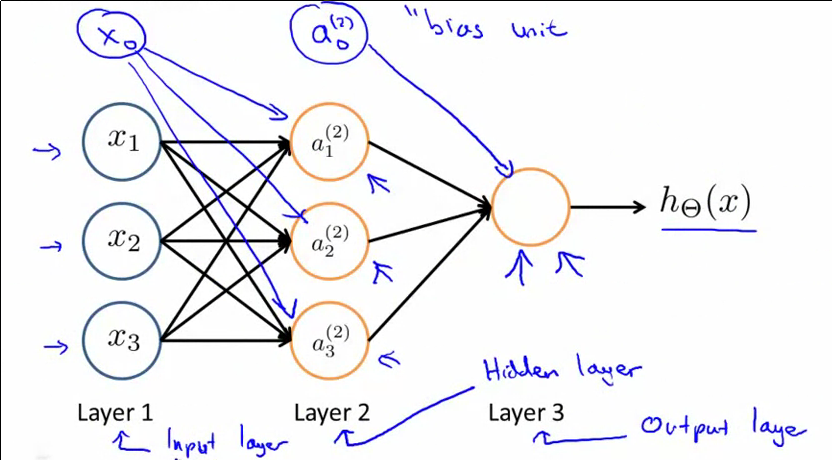
\includegraphics[width=0.7\columnwidth]{Figs/neunet.png}
\caption{\label{fig:neunet} Representation of a feedforward neural
  network. Capture from the A. Ng lecture.}
\end{figure}

We will denote $a_i^{(j)}$ the activation of the i-th unit of j-th
layer. We denote $\theta^{(j)}$ the matrix of weights from layer $j$
to layer $j+1$\footnote{We here consider only feedforward neural
  networks were the connections always go from layer $j$ to layer
  $j+1$}. The activation is computed according to~:
\begin{equation}
\begin{cases}
\forall i \geq 1, \forall j>1, a_i^{(j)} &= g(z_i^{(j)})\\
\forall i \geq 1, \forall j>1, z_i^{(j)} &= \sum_k \theta_k^{(j-1)} a_k^{(j-1)}\\
\forall i \geq 1, a_i^{(1)} &= x_i\\
\forall j, a_0^{(i)} &= 1
\end{cases}
\end{equation}
These equations tell nothing more than that the first neuron is the
bias for the next layer, the activations $a_i^{(1)}$ of the first layer equal our
inputs and each neuron in a subsequent layer computes its activation $a_i^{(j)}$
as a sigmoid of a weighted sum of the activations of the previous
layer $a_k^{(j-1)}$. A vectorized notation for computing the activations of layer
$j+1$ is simply $a^{(j+1)} = g(\theta^{(j)} . a^{(j)})$ where
$\theta^{(j)}$ is a matrix of size $|L_{j+1}| \times |L_{j}|$ with
$|L_j|$ the number of neurons in layer $j$ (the bias being
included). For regression, the last layer contains a single neuron of
which the activation, if unfolded, is a function of the input
$x$. Computing the activations in a layer-wise manner from the very
first layer to the output is called the forward propagation. If we
take a closer look to the 3-layers neural network depicted above, the
hidden to output layer is nothing more than a logistic regression with
Layer 2 representing the features. Now, if we include the very first
layer with the weights projecting the inputs to the hidden layer, we
can see it as building the features feeding the logistic
regression. And the nice thing there is that the features are learned
through the weights from Layer 1 to Layer 2. It may not be completely
clear that the features we compute that way (the activations of layer
1) can be arbitrary polynomials but indeed one may demonstrate that if
we don't restrict ourselves to a single hidden layer, one can
approximate any function (feedforward neural networks are universal
approximators) so that feedforward neural networks have at least the
expressiveness of logistic regression.\\


\textbf{Ref pour l'approximateur universel?}



\end{document}
